%----------------------------------------------------------------
%
%  File    :  curriculumvitae.tex
%
%  Authors :  Philipp Schunker
% 
%  Created :  28 Jun 2019
% 
%  Changed :  28 Jun 2019
% 
%----------------------------------------------------------------

% --- General Setup ---------------------------------------------

\documentclass[11pt,a4paper,oneside]{scrbook}

% select correct document language here
\usepackage[ngerman]{babel}
%\usepackage[english]{babel}

% for nicer PDF rendering. Alternatively, when using MikTeX,
% you could also manually install the cm-super package  
\usepackage{lmodern}

\usepackage[utf8]{inputenc}
\usepackage[T1]{fontenc}

% for Arial uncomment next two lines...
%\usepackage{uarial}
\usepackage{}
\renewcommand{\familydefault}{\sfdefault}
\usepackage{helvet}

\usepackage[bf,sf]{subfigure}
\renewcommand{\subfigtopskip}{0mm}
\renewcommand{\subfigcapmargin}{0mm}

% --- General Packages ----------

\usepackage{url}
\usepackage{latexsym}
\usepackage{geometry} % define pagesize in more detail
%\usepackage{fancyhdr} % nicer headers and footers	%commented
\usepackage{colortbl} % define colored backgrounds for tables
\usepackage{courier} %for listings
\usepackage{listings} % nicer code formatting
\lstset{basicstyle=\ttfamily,breaklines=true}
\usepackage[pdftex]{graphicx}
\DeclareGraphicsExtensions{.pdf,.jpg,.png}
\pdfcompresslevel=9
\pdfpageheight=297mm
\pdfpagewidth=210mm
\usepackage[         % hyperref should be last package loaded
    pdftex,
    bookmarks,
    bookmarksnumbered,
    linktocpage,
    pagebackref,
    pdfview={Fit},
    pdfstartview={Fit},
    pdfpagemode=UseOutlines,                 % open bookmarks in Acrobat
  ]{hyperref}
\usepackage{bookmark}
\usepackage{lastpage}

%\KOMAoptions{headsepline=true}
%\AddToLayerPageStyleOptions{scrheadings}
%{oninit={% will be excecuted whenever the output of the layers is initialized
    %\ifstr{\headmark}{}{\KOMAoptions{headsepline=false}}{}%
%}}

\geometry{a4paper,left=30mm,right=25mm, top=30mm, bottom=30mm}

\setlength{\parskip}{3pt plus 1pt minus 0pt}       % vert. space before a paragraph
%\setlength\leftmargini{0em}
%\setlength\LTleft{0pt}
%\setlength\LTright{0pt}

\setcounter{tocdepth}{1}        % lowest section level entered in ToC
\setcounter{secnumdepth}{2}     % lowest section level still numbered

%---
%\usepackage{scrlayer-scrpage}
\usepackage[automark]{scrlayer-scrpage} % sets pagestyle scrheadings automatically
\setkomafont{pageheadfoot}{\normalfont\normalcolor}
\clearscrheadfoot	%deprecated
\clearpairofpagestyles
%\lehead{Lebenslauf Philipp Schunker}
\ohead{Lebenslauf Philipp Schunker}
%\ohead{}
\ofoot{\pagemark/\pageref*{LastPage}}
%---

% --- Custom Packages ----------

\usepackage{verbatim}
\usepackage[export]{adjustbox}
\usepackage{array}
\usepackage{longtable}%[v=4.13]
\usepackage{tabu}
\usepackage{tabularray}
\usepackage[table]{xcolor}
\usepackage{enumitem}
\usepackage{booktabs}
\usepackage{etoolbox}
\usepackage{hyperref}

%\definecolor{tableHeader}{RGB}{211, 47, 47}
\definecolor{tableHeader}{RGB}{0, 122, 255}
\definecolor{tableLineOne}{RGB}{245, 245, 245}
\definecolor{tableLineTwo}{RGB}{224, 224, 224}

\newcommand{\tableHeaderStyle}{
    \rowfont{\leavevmode\color{white}\bfseries}
    \rowcolor{tableHeader}
    \setlength{\tabcolsep}{0pt}
    \renewcommand{\arraystretch}{0}
}

% --- \textbullet\ text ----------

\newlength\boxwid%  
\let\oldtextbullet=\textbullet
\def\textbullet{%
    \settowidth{\boxwid}{\indent\oldtextbullet\ }%
    \hangindent=\boxwid%
    \oldtextbullet}
    
% --- \tabitem text ----------

%\newcommand{\tabitem}{~~\llap{\textbullet}~~}
\newcommand{\tabitem}{{\textbullet}~}

\begin{comment}
\setlist[tabitem]{nosep,
        topsep= 0pt,
        partopsep=0pt,
        leftmargin= *,
        label=\textbullet,
        before=\vspace{-0.6\baselineskip},
	after=\vspace{-\baselineskip}
}
\end{comment}

% --- \hangbullet{text} ----------

\newcommand\hangbullet[1]{\leftskip1.5\parindent
\hspace*{-\parindent}\llap{{\textbullet\enspace}}#1\par\leftskip0pt}
%\hspace*{-\parindent}\leavevmode\llap{{\textbullet\enspace}}#1\par\leftskip0pt}

% --- Longtabu Settings ----------

\taburowcolors[2] 2{tableLineOne .. tableLineTwo}
\tabulinesep = ^0.5mm_0.3mm
\everyrow{\tabucline[.05mm white]{\dimexpr\tabcolsep+0.1pt\relax}}

\AtBeginEnvironment{tabu}{\setlist[itemize]{wide = 0pt, nosep, leftmargin = *}}

\makeatletter
\newcommand*{\compress}{\@minipagetrue}
\makeatother

% --- Start of Document ----------------------------------------


\begin{document}

%\frontmatter
%\normalsize
%\pagestyle{empty}            % for title pages

% include correct title, depending on language
%\pagestyle{fancy}
%\fancyhead{}		%commented
%\fancyfoot{}	%page numbering in lower right corner
\setlength{\headheight}{15pt}
%\renewcommand{\headrulewidth}{0.0pt}		%commented
%\fancyfoot[R]{\thepage}
%\pagenumbering{roman}        % for preliminary pages

\mainmatter

\cleardoublepage
%\renewcommand{\headrulewidth}{0.4pt}		%commented
%\pagestyle{fancy}            % for main pages	%commented
\pagestyle{scrheadings}
%\fancyhead[RO]{\slshape \nouppercase{\leftmark}}
%\fancyfoot[R]{\thepage}
%\pagenumbering{arabic}      % for main pages

%--- Include your chapters here ----------

%----------------------------------------------------------------
%
%  File    :  curriculumvitae-main.tex
%
%  Authors :  Philipp Schunker
% 
%  Created :  28 Jun 2019
% 
%  Changed :  28 Jun 2019
% 
%----------------------------------------------------------------

\thispagestyle{empty}

\begin{comment}
\begin{figure}[htbp]
	%\centering
	
\includegraphics[height=5cm]{images/philipp}
\end{figure}
\end{comment}

\begin{minipage}{0.7\textwidth}
%Lebenslauf\\
\begin{addmargin}[2em]{2em}% 1em left, 2em right
\Large{\textbf{Lebenslauf}}\vspace{0.1cm}\\
\Large{\textbf{Philipp Schunker}}\vspace{1.0cm}\\
%\small{philipp@schunker.at}\vspace{0.5cm}\\
\end{addmargin}
\end{minipage}
\begin{minipage}{0.3\textwidth}
%\begin{figure}[htbp]
	%\centering
	 %
\includegraphics[width=0.6\textwidth]{images/philipp}
	 
\includegraphics[width=\textwidth]{images/philipp}
%\end{figure}
\end{minipage}

\begin{comment}
\begin{table*}[htbp]
	\centering
		\begin{tabular}{|l|c|r|}
		%\hline
		%\rowcolor[gray]{0.9}
		%Spalte 1 & Spalte 2 & Spalte 3 \\
		\hline
		Affen & Giraffen & Löwen \\
		Äpfel & Birnen & Bananen \\
		Irgend & et & was \\
		\hline
		\end{tabular}
\end{table*}
\end{comment}

\begin{comment}
\begin{tabular*}{\textwidth}{c @{\extracolsep{\fill}} ccccc}
		\hline
		Affen & Giraffen & Löwen \\
		Äpfel & Birnen & Bananen \\
		Irgend & et & was \\
		\hline
\end{tabular*}
\end{comment}

\begin{comment}
\begin{longtabu} to \textwidth {l >{\bfseries}X[r, 2] X[4] l}
	\tableHeaderStyle
	& Angaben zur Person & & \\
        & Vorname Nachname & Philipp Schunker & \\
        & Staatsangehörigkeit & Österreich & \\
        & Geburtsdatum & 18.09.1991 & \\
        & Geschlecht & Männlich & \\
        	\tableHeaderStyle
	& Gewünschtes Berufsfeld & Leitender Software-Entwickler und Software-Architekt &\\
	\tableHeaderStyle
	& Berufserfahrung & & \\
	& Datum & November 2013 bis heute & \\
        & Funktion & IT Systems Engineer & \\
        & Arbeitgeber & Allianz Technology GmbH & \\
        & Tätigkeitsbereich & IT Operations - Application and System Services & \\ \bottomrule
        %----
        	& Datum & Juni 2013 bis Oktober 2013 & \\
        & Funktion & Junior Software Developer & \\
        & Arbeitgeber & Österreichisches Bundesheer, Führungsunterstützungzentrum Abteilung FüUZ/Applikation & \\
        & Tätigkeitsbereich & Applikationsentwicklung Intranet & \\ \bottomrule
        %----
        	& Datum & November 2011 bis Mai 2012 & \\
        & Funktion & Programmierer im Präsenzdienst & \\
        & Arbeitgeber & Österreichisches Bundesheer, Führungsunterstützungzentrum Abteilung FüUZ/Applikation & \\
        & Tätigkeitsbereich & Automatisierung der Qualitätssicherung von Webapplikationen & \\\bottomrule
        %----
        	& Datum & August 2010 bis September 2010 & \\
        & Funktion & Urlaubsaushilfe & \\
        & Arbeitgeber & Österreichische Post AG, Zustellbasis 1140 Wien & \\
        & Tätigkeitsbereich & Post-Zusteller & \\ \bottomrule
        %----
        	& Datum & Juli 2009 bis August 2009 & \\
        & Funktion & Berufspraktikum & \\
        & Arbeitgeber & 
        \begin{itemize}
	\item Service, Wartung und Instandsetzung von Computerhardware
	\item Entwicklung und Betreuung der intern genutzten Software und IT-Infrastruktur
	\end{itemize} & \\
        & Tätigkeitsbereich & Post-Zusteller & \\ \bottomrule
\end{longtabu}
\end{comment}

%\begin{longtable}{rl}
\begin{longtabu} to \textwidth {>{\bfseries}X[r, 2] X[4]} %rl
	\tableHeaderStyle
	\large{Angaben zur Person} & \\
        Vorname Nachname & Philipp Schunker \\
        Staatsangehörigkeit & Österreich \\
        Geburtsdatum & 18.09.1991 \\
        Geschlecht & Männlich \\
        E-Mail & philipp@schunker.at \\
        Telefonnummer & +43 699 1946 7200 \\
	Gewünschtes Berufsfeld & Leitender Software-Entwickler und Software-Architekt \\
	\tableHeaderStyle
	\large{Berufserfahrung} & \\
	Datum & November 2013 bis heute \\
        Funktion & IT Systems Engineer \\
        Arbeitgeber & Allianz Technology GmbH \\
        Tätigkeitsbereich & IT Operations - Application and System Services \\ \bottomrule
        %----
        	Datum & September 2018 bis heute \\
        Funktion & Frei- und nebenberuflicher Software-Entwickler \\
        Tätigkeitsbereich & App-Entwicklung \\ 
	% & \begin{tabular}{cc}
	Veröffentlichungen & \begin{tabular}{m{.2\textwidth} m{.2\textwidth} }
	MapReminder & 
\includegraphics[height=1.0cm]{images/iOS-MapReminder-1024} \\
	\end{tabular} \\
	& MapReminder ist eine leicht zu bedienende und im App Store verfügbare iOS App für ortsbezogene Erinnerungen \\ 
	& Diverse Open Source Software-Projekte auf GitHub \\ \bottomrule
        %----
        Datum & Juni 2013 bis Oktober 2013 \\
        Funktion & Junior Software Developer \\
        Arbeitgeber & Österreichisches Bundesheer, Führungsunterstützungzentrum Abteilung FüUZ/Applikation \\
        Tätigkeitsbereich & Applikationsentwicklung Intranet \\ \bottomrule
        %----
        	Datum & November 2011 bis Mai 2012 \\
        Funktion & Programmierer im Präsenzdienst \\
        Arbeitgeber & Österreichisches Bundesheer, Führungsunterstützungzentrum Abteilung FüUZ/Applikation \\
        Tätigkeitsbereich & Automatisierung der Qualitätssicherung von Webapplikationen \\ \bottomrule
        %----
        	Datum & August 2010 bis September 2010 \\
        Funktion & Urlaubsaushilfe \\
        Arbeitgeber & Österreichische Post AG, Zustellbasis 1140 Wien \\
        Tätigkeitsbereich & Post-Zusteller \\ \bottomrule
        \newpage
        %----
        Datum & Juli 2009 bis August 2009 \\
        Funktion & Berufspraktikum \\
        Arbeitgeber & Audio Video Media Service GmbH \\
	Tätigkeiten und Zuständigkeiten &
	%\tabitem Service, Wartung und Instandsetzung von Computerhardware \newline
	%Service, Wartung und Instandsetzung von Computerhardware \newline
	%\hangbullet{Entwicklung und Betreuung der intern genutzten Software und IT-Infrastruktur} \\
	%Entwicklung und Betreuung der intern genutzten Software und IT-Infrastruktur \\
	%\compress
	\begin{itemize}[nosep,leftmargin=1em] 
	\item Service, Wartung und Instandsetzung von Computerhardware
    	\item Entwicklung und Betreuung der intern genutzten Software und IT-Infrastruktur
	\end{itemize} \\
        Tätigkeitsbereich & Informations- und Kommunikationstechnik \\ \bottomrule
        %----
        Datum & Juli 2007 bis August 2007 \\
        Funktion & Berufspraktikum \\
        Arbeitgeber & Audio Video Media Service GmbH \\
	Tätigkeiten und Zuständigkeiten &
	%\tabitem Service, Wartung und Instandsetzung von Computerhardware \newline
	%\textbullet{Entwicklung und Betreuung der intern genutzten Software und IT-Infrastruktur} \\
	%\compress
	\begin{itemize}[nosep,leftmargin=1em]
	\item Service, Wartung und Instandsetzung von Computerhardware
    	\item Entwicklung und Betreuung der intern genutzten Software und IT-Infrastruktur
	\end{itemize} \\
        Tätigkeitsbereich & Informations- und Kommunikationstechnik \\ \bottomrule
        	\tableHeaderStyle
	\large{Schul- und Berufausbildung} & \\
	%----
    Datum & September 2016 bis September 2019 \\
    Name und Art der Bildungs- oder Ausbildungseinrichtung & University of Applied Sciences FH Campus Wien \newline
    Bachelorstudiengang Informationstechnologie und Telekommunikationstechnik \\
    Bezeichnung der erworbenen Qualifikation & Bachelor of Science in Engineering (BSc) \\
    Publikationen &
    \begin{itemize}[nosep,leftmargin=1em]
	\item Bachelorarbeit 1: Pfadsuche basierend auf Reinforcement Learning und Monte-Carlo Tree Search
	\item Bachelorarbeit 2: Entscheidungsfindung basierend auf der Monte-Carlo Tree Search und künstlichen neuronalen Netzen
    	\item Telekommunikation: Car-to-Car Communication 
	%\scriptsize{\url{https://schunker-my.sharepoint.com/personal/philipp_schunker_at/_layouts/15/onedrive.aspx?id=\%2Fpersonal\%2Fphilipp\%5Fschunker\%5Fat\%2FDocuments\%2FAnlagen\%2FCar2CarCommuncation\%2Epdf&parent=\%2Fpersonal\%2Fphilipp\%5Fschunker\%5Fat\%2FDocuments\%2FAnlagen}}
	\item Internationalisierung@Home: What programming and logic have in common and how to write error-free software 
	%\scriptsize{\url{https://schunker-my.sharepoint.com/personal/philipp_schunker_at/_layouts/15/onedrive.aspx?id=\%2Fpersonal\%2Fphilipp\%5Fschunker\%5Fat\%2FDocuments\%2FAnlagen\%2FFunctionalProgramming\%2Epdf&parent=\%2Fpersonal\%2Fphilipp\%5Fschunker\%5Fat\%2FDocuments\%2FAnlagen}}
	\end{itemize} \\ 
	Projekte & 
	\begin{tabular} {m{.4\textwidth} m{0.05\textwidth} }
	\begin{itemize}[nosep,leftmargin=0.5em,topsep=10pt]
		\item VienNav (MTCSNav) Praktische Umsetzung für die Verifizierung und Auswertung der in der Bachelorarbeit 1 dargelegten Theorie
	\end{itemize}
	& 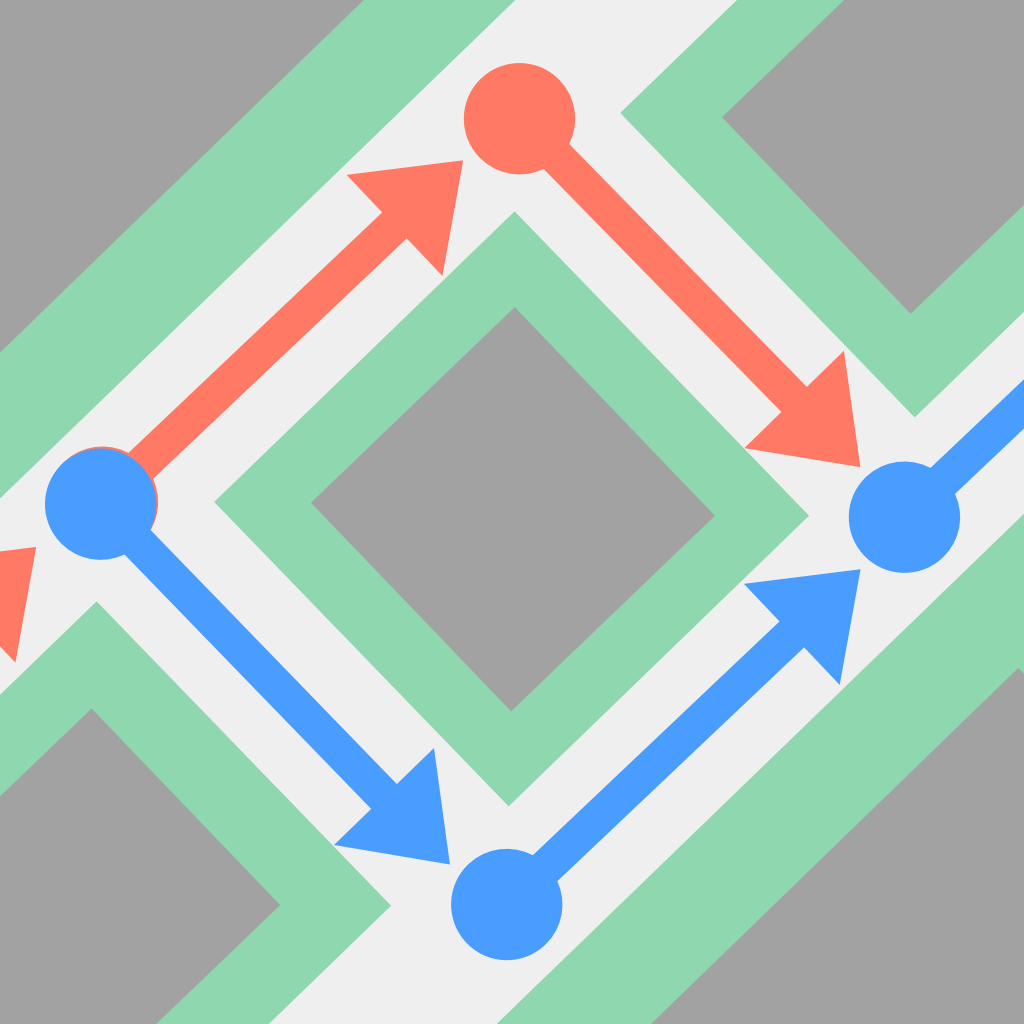
\includegraphics[height=1.0cm]{images/MCTS-Icon-1024} \\
	\begin{itemize}[nosep,leftmargin=0.5em]
		\item MLChess Praktische Umsetzung für die Verifizierung und Auswertung der in der Bachelorarbeit 2 dargelegten Theorie
	\end{itemize}
 	& 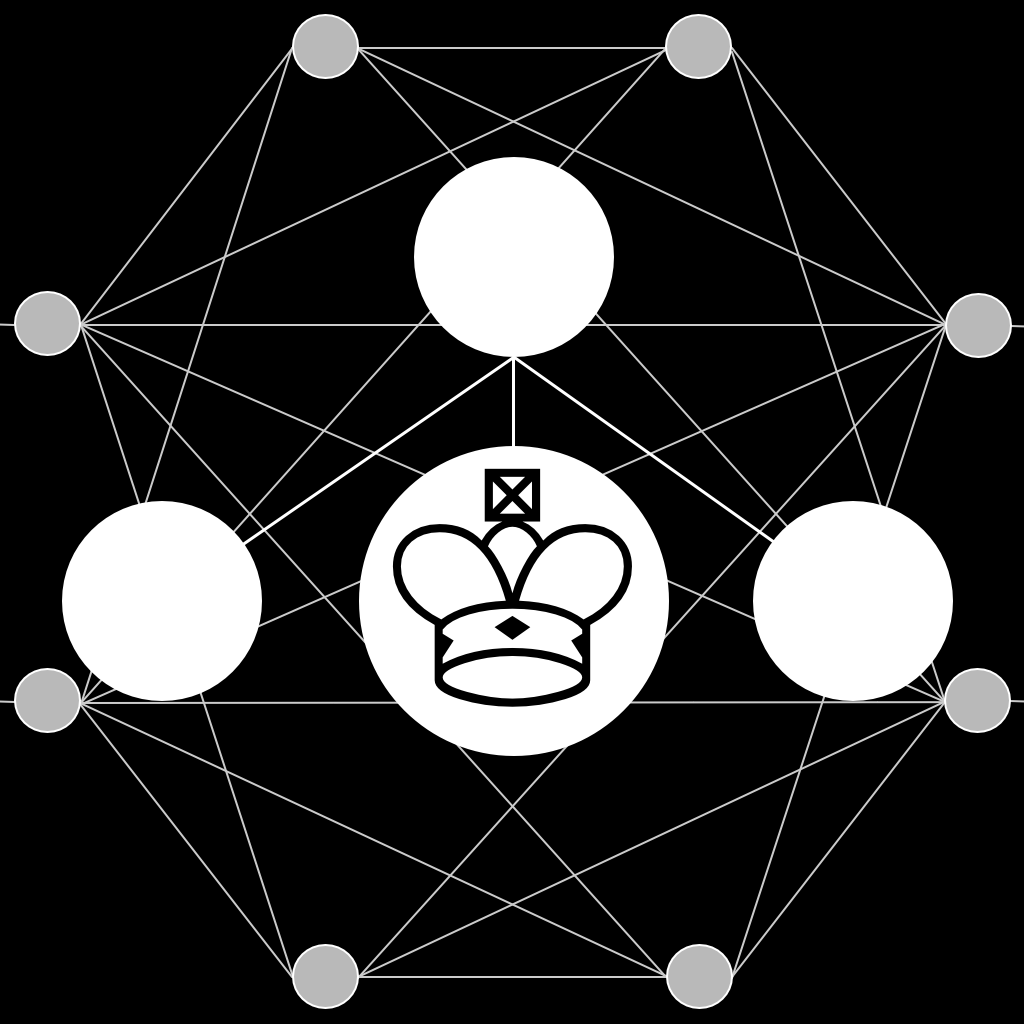
\includegraphics[height=1.0cm]{images/MLChess-Icon-1024} \\
	\end{tabular} \\
	%& Praktische Umsetzung für die Verifizierung und Auswertung der in der Bachelorarbeit 1 dargelegten Theorie \\
	\bottomrule
	\newpage
    %----
    Datum & Oktober 2012 bis Mai 2013 \\
    Name und Art der Bildungs- oder Ausbildungseinrichtung & FH des bfi Wien Bachelorstudiengang Projektmanagement und IT \\ \bottomrule
    %----
    Datum & September 2006 bis Juni 2011 \\
    %Name und Art der Bildungs- oder Ausbildungseinrichtung & Höhere Technische Bundeslehranstalt Wien 16 \\
	Name und Art der Bildungs- oder Ausbildungseinrichtung & Höhere Technische Bundeslehranstalt Wien 16 \newline
	Informationstechnologie \newline mit Schwerpunkt Netzwerktechnik\\
    Bezeichnung der erworbenen Qualifikation & Diplom- und Reifeprüfung \\
    \bottomrule
    %Bezeichnung der Qualifikation & Abteilung Informationstechnologie mit Schwerpunkt Netzwerktechnik \\ 
    %\bottomrule
    %----
    Datum & September 2002 bis Juli 2006 \\
    Name und Art der Bildungs- oder Ausbildungseinrichtung & Bundesrealgymnasium Wien 8 Albertgasse Unterstufe \\ \bottomrule
    %----
    Datum & September 1998 bis Juli 2002 \\
    Name und Art der Bildungs- oder Ausbildungseinrichtung & Volksschule Wien 16 Grubergasse \\ 	\bottomrule
    %----
    Muttersprache & Deutsch \\
	Sonstige Sprache(n) & Englisch \\ %\bottomrule
	Selbstbeurteilung Englisch &
	%\begin{tabular}{| c | c | c | }
	\begin{tabular}{| c | c | c | c | c | c |}
	\hline
	%Verstehen & Sprechen & Schreiben \\
	%B2 & B2 & B2 \\
	\multicolumn{2}{| c |}{Verstehen} & \multicolumn{2}{| c |}{Sprechen} & \multicolumn{2}{| c |}{Schreiben} \\
	\hline
	Hören & Lesen & \multicolumn{2}{| c |}{} & \multicolumn{2}{| c |}{} \\
	\hline
	\multicolumn{2}{| c |}{C1} & \multicolumn{2}{| c |}{B2} & \multicolumn{2}{| c |}{B2} \\
	\hline
	\end{tabular} \\
	\bottomrule
	%----
    Soziale Fähigkeiten und Kompetenzen &
	\tabitem Teamfähig \newline
	\tabitem Motiviert \newline
	\tabitem Freundlich \newline
	\tabitem Objektiv \\ \bottomrule
	%---
	Organisatorische Fähigkeiten und Kompetenzen &
	\tabitem Agile Scrum Foundation Zertifizierung \newline
	\tabitem Ziel- und leistungsorientierte Arbeitsweise \newline
	\tabitem Körperliche und geistige Belastbarkeit \newline
	\tabitem Solides und kompetentes Auftreten \newline
	\tabitem Zuverlässigkeit, Engagement und Flexibilität \\ \bottomrule
	%---
	Technische Fähigkeiten und Kompetenzen &
	\begin{itemize}[nosep,leftmargin=1em]
	\item Programmierung von Software in imperativen und objektorientierten Sprachen: C, Java, C\#, Objective-C, Swift
	\item Erfahrung in der Entwicklung von Software sowie im Aufbau und Betrieb von IT-Dienstleistungen
	\item Erfahrung im Bereich der Qualitätssicherung durch meine Tätigkeit im Präsenzdienst
	\item Betriebssysteme: Windows, Linux, macOS, iOS, Android
	\item Hervorragende Office-Kenntnisse im Umgang mit Word, Excel, Powerpoint, Access sowie VBA-Programmierung
	\item Netzwerkmanagement: Netzwerkaufbau, Netzwerkplanung und Netzwerkkomponenten
	\item Verteilte Computersysteme und Client-Server Architekturen: LDAP-, DHCP-, Datenbank-, Mail-, Terminal-, Print- und Web-Server
	\item IT-Security: Symmetrische (DES, AES) und asymmetrische (RSA, Elgamal) Verschlüsselungsverfahren, Schlüsselaustauschverfahren (Diffie-Hellman)
	\item Datenbanksysteme: Aufbau, Funktionsweise, Anbindung und Entwicklung mit SQL
	\item Web-Technologien: Entwicklung mit statischen und dynamischen Technologien wie HTML, CSS, php, Javascript und React
	\item Telekommunikation und IoT: GSM, UMTS, LTE, 5G, Modulations- und Übertragungsverfahren %\\ \bottomrule
	\end{itemize} \\
	Künstlerische Fähigkeiten und Kompetenzen &
	\tabitem Photographie \newline
	\tabitem Bildbearbeitung \\ \bottomrule
	Hobbies, Interessen und Freizeitaktivitäten &
	\tabitem Programmieren \newline
	\tabitem Reisen \newline
	\tabitem Sport (Fußball, Laufen, Mountainbiken, Snowboarden) \newline
	\tabitem Filme und Musik \\ \bottomrule
	Weitere Informationen &
	MapReminder im App Store \newline
	\small{\url{https://itunes.apple.com/us/app/mapreminder/id1437456241?l=de&ls=1&mt=8}} \newline
	VienNav im Testflight Programm \newline
	\small{\url{https://testflight.apple.com/join/kxyfo2nV}} \newline
	GitHub Account und Projekte \newline
	\small{\url{https://github.com/philsch91}} \newline
	Car-to-Car Communication \newline
	\small{\url{https://schunker-my.sharepoint.com/personal/philipp_schunker_at/_layouts/15/onedrive.aspx?id=\%2Fpersonal\%2Fphilipp\%5Fschunker\%5Fat\%2FDocuments\%2FAnlagen\%2FCar2CarCommuncation\%2Epdf&parent=\%2Fpersonal\%2Fphilipp\%5Fschunker\%5Fat\%2FDocuments\%2FAnlagen}} \newline
	What programming and logic have in common and how to write error-free software \newline
	\small{\url{https://schunker-my.sharepoint.com/personal/philipp_schunker_at/_layouts/15/onedrive.aspx?id=\%2Fpersonal\%2Fphilipp\%5Fschunker\%5Fat\%2FDocuments\%2FAnlagen\%2FFunctionalProgramming\%2Epdf&parent=\%2Fpersonal\%2Fphilipp\%5Fschunker\%5Fat\%2FDocuments\%2FAnlagen}} \newline
%\end{longtable}
\end{longtabu}
          % main

\end{document}

